% ch-concentration.tex -- theory: the two concentration models, material properties, boundary conditions
\chapter{Concentration and boundary conditions}
\label{ch:concentration}

Two things remain to be explained about the model: how the solute is
transported, and what happens at the edges of the domain. They are grouped here
because both are choices you make in the input file that change the answer
rather than merely the cost, and because both are easy to make carelessly.

Yuzen offers two concentration models. \val{"WM"} is well mixed and treats the
concentration as uniform across the film thickness; \val{"CZ"} resolves the
distribution through the thickness. Both are available in one and two
dimensions. The first supports every physics term; the second gives up two of
them. Which one is right
depends on a single dimensionless number, and \cref{sec:conc:wm} says which.

\section{The well-mixed model}
\label{sec:conc:wm}

\key{Physics.ConcField.Model = "WM"} assumes the concentration is uniform
across the thickness. There is one unknown $c(x,y,t)$ per point and no mesh in
the thickness direction at all, which is what makes the model cheap. It solves
\cref{eq:conc-dim}.

The assumption is sound when diffusion across the thickness is much faster than
evaporation removes solvent from the surface, that is, when the P\'eclet number

\[
  \Pen = \frac{E_0 h_0}{D_0}
\]

is small. A thin film of a low-viscosity solvent that dries slowly is well
mixed to a very good approximation.

When $\Pen$ is not small the assumption fails, and it fails in a specific and
consequential way. Only the region near the free surface becomes concentrated,
and in reality that region forms a hard skin which then slows all subsequent
drying. The well-mixed model cannot represent this at all. Its errors follow
from one another:

\begin{itemize}
  \item there is no skin, because there is no cross-film structure to form one
    from, so drying does not slow down when it should;
  \item the surface concentration is \textbf{under-predicted}, since the
    solute that should have accumulated at the surface has been averaged over
    the whole thickness;
  \item the rise in viscosity is therefore weaker than it should be, because
    the exponential law of \cref{eq:prop-mu} is evaluated at too low a
    concentration;
  \item and the Marangoni stress is weaker too, because it is driven by the
    surface concentration gradient, which has been smoothed away.
\end{itemize}

Note that these are not independent errors that might partly cancel: they all
come from the same missing structure and all push in the same direction,
toward a film that stays more mobile for longer than the real one.

The equation is solved as the balance of the solute $hc$ of each cell: the
solute that crosses a face is the concentration there times the very volume
flux the film-height equation puts through that face in the same step, so the
solute of a closed film is kept to rounding, with evaporation or without, and
a uniform concentration stays uniform whatever the film does
(\cref{sec:disc:wm-conservative}). $c$ is kept within $[0, 1]$ by moving
solute between cells, never by cutting it (\cref{sec:disc:convection}).

\key{EnableConvection} and \key{EnableDiffusion} switch off the convective and in-plane
diffusive terms individually, which is useful for isolating one mechanism in a
test but is not a physical setting.

\section{The \texorpdfstring{\val{"CZ"}}{CZ} model: resolving the thickness direction}
\label{sec:conc:cz}

\key{Physics.ConcField.Model = "CZ"} solves for the concentration with the
thickness direction resolved: $c(x,z,t)$ with \key{Grid.Dimension = "xh"}, and
$c(x,y,z,t)$ with \key{Grid.Dimension = "xyh"}, which is the pseudo-3D case ---
the film spreads in $x$ and $y$ while the concentration is also resolved
across it. The film is mapped onto a fixed coordinate $\zeta \in [0,1]$, so
that as the film thins the $\zeta$ mesh contracts with it and the number of
cells through the thickness stays constant. That number is \key{Grid.Nz}.

Both dimensions are handled by the same code; the film's dimension is decided
by the grid, and with $N_y = 1$ no $y$ term is formed at all. The two-dimensional
case adds the mixed $x$--$y$ terms to the film-height equation and the
$y$--$\zeta$ cross terms to the concentration equation. \file{concz\_2d.toml}
is a worked example.

The boundary conditions in $\zeta$ are what make the model do its job. The
concentration equation is solved in conservative form for $hc$ on the $\zeta$
grid: each cell exchanges solute through face fluxes, and the flux through its
$\zeta$ faces follows from the discrete conservation of the grid with the
film's step, so a uniform concentration stays uniform and the solute of a
closed film is kept to rounding. No solute crosses the substrate or the free
surface: the total flux there, the advection by the evaporating solvent and
the whole diffusive flux, including its part along the slope of the surface
or the substrate, is zero. The solvent that leaves the top cell without its
solute is what builds up the concentrated layer near the surface. The rate of
evaporation itself is evaluated with \textbf{the free-surface concentration},
not the depth average, which is the whole point: it is what allows the surface
layer to slow its own drying, the effect the well-mixed model is missing.

\begin{figure}[tbp]
  \centering
  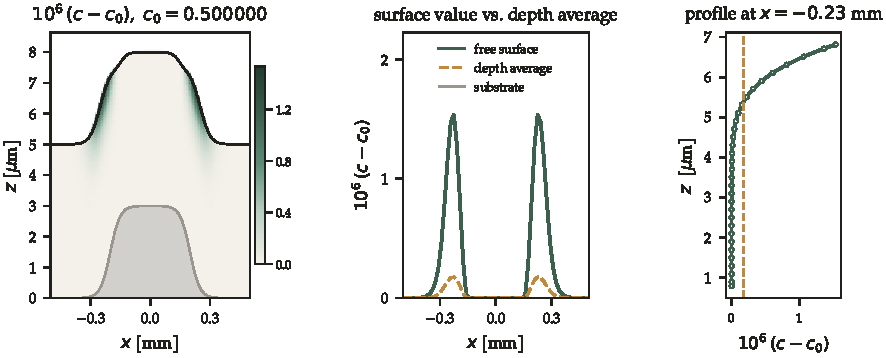
\includegraphics[width=\textwidth]{../figures/concz.pdf}
  \caption{What the \val{"CZ"} model resolves that the well-mixed one cannot,
    from \file{concz\_2d.toml} on the plane $y = 0$ at the end of the run.
    \textbf{Left:} the film over the substrate relief, colored by $c$ less
    the value $c_0$ it started at; the departure is in the seventh decimal.
    The solute sits in
    a layer hugging the free surface, and it is visible on the two shoulders
    and nowhere else. \textbf{Center:} the free-surface value, the depth average and the
    substrate value along $x$. They separate sharply at the two places where
    the film is thinnest, because the same evaporative flux is concentrated
    into less liquid there; everywhere else they are indistinguishable.
    \textbf{Right:} the profile through the thickness at that point, on the
    $\zeta$ grid the model uses, with the depth average marked. A well-mixed
    run carries only the dashed value, and it is the solid curve's top point
    that sets the surface tension and the evaporation rate.
    \key{Fluid.\bk Diffusivity} in that case is set below the value the 1-D
    cases use, on purpose: raise it back and diffusion halves the step.
    How far below is a measured choice
    rather than a free one, because the layer is about $\sqrt{D t}$ deep and
    the cells are \SI{0.2}{\micro\metre} high. At \num{3e-10} the layer spans
    four cells and the height of the step converges at second order in the
    cell height; two orders lower it is thinner than one cell and the step
    scales with the mesh instead. The case file carries the
    numbers.\label{fig:conc:czprofile}}
\end{figure}

Two further consequences follow from letting the viscosity vary through the
thickness. The in-plane velocity can no longer be written down analytically as
a parabola, so it is constructed by integrating $1/\mu$ and $z/\mu$ numerically
across the thickness. And the film thickness itself is then advanced with the depth integral of
that profile as its flux --- the kinematic condition at the free surface ---
rather than with a closed-form one; the surface tension in it is that of the
surface concentration.

The costs are real and you should weigh them before choosing this model. The
number of concentration unknowns grows from $N_x$ to $N_x \times N_z$. More
importantly, the set of physics terms available shrinks:

\begin{warn}[\val{"CZ"} has no disjoining pressure and no source term]
  The terms \val{"CZ"} supports are capillary pressure, solutal capillarity,
  vertical gravity, in-plane gravity, centrifugal force and evaporation.
  \key{Physics.DisjoiningPressure} and the whole of \key{Physics.Source} are
  \textbf{not available}, and are ignored without a diagnostic
  (\cref{sec:ref-physics:disjoining}). Since disjoining pressure is what
  produces a contact line, \textbf{every contact-line problem must use}
  \val{"WM"}. There is no way to combine a resolved cross-film concentration
  with a moving contact line in the present solver.
\end{warn}

\section{Concentration dependence of the material properties}
\label{sec:conc:properties}

The \key{Fluid} block gives each property at a reference concentration
\key{BaseConc} and the law by which it varies away from it
(\cref{sec:ref-domain:fluidconc}):

\begin{align}
  \sigma(c) &= \mathrm{BaseValue}
    + \mathrm{Coef}\,(c - \mathrm{BaseConc}),
    \label{eq:prop-sigma}\\
  \mu(c) &= \mathrm{BaseValue}\,
    \exp\bigl(\mathrm{Exponent}\,(c - \mathrm{BaseConc})\bigr),
    \label{eq:prop-mu}\\
  D(c) &= \mathrm{BaseValue}\,
    \exp\bigl(\mathrm{Exponent}\,(c - \mathrm{BaseConc})\bigr).
    \label{eq:prop-diff}
\end{align}

Surface tension is linear in concentration; viscosity and diffusivity are
exponential.

\Cref{eq:prop-mu} is the strongest non-linearity in the solver, and it is worth
being specific about how strong. \key{Fluid.Viscosity.Exponent} can reasonably
be around 10, and at that value \textbf{a change in concentration of 0.1
multiplies the viscosity by $e$}. Over the course of a drying run the
concentration may move by several tenths, so the viscosity can rise by orders
of magnitude. This is not a numerical inconvenience --- it is the physics of
the film solidifying and the flow stopping --- but it is also the reason the
Newton iteration and the time-step controller have to work hardest late in a
drying run (\cref{ch:convergence,ch:timeintegration}).

The coupling closes in both directions, and through more than one route.
\Cref{eq:prop-sigma} feeds two places at once: its slope \key{Coef} is the
Marangoni number $\Ma$ that drives \cref{eq:q-sc}, and $\sigma(c)$ also sits in
the mobility of the capillary-pressure term \cref{eq:q-cap}, so drying changes
how fast the film levels even with the Marangoni stress switched off. Viscosity
enters \emph{every} flux term through $\mu(c)$. So the concentration field
determines the flow, while the flow --- through convection in
\cref{eq:conc-dim}, and through the thickness that divides the evaporation term
of \cref{eq:conc-adv}
--- determines the concentration field. The two equations are coupled both
ways, which is why they are solved together rather than in sequence.

\section{What the boundary conditions mean physically}
\label{sec:conc:boundaries}

The height equation is fourth order, so \textbf{each boundary needs two
conditions, not one}. That is why you choose a named type rather than writing a
value: each name stands for a pair. The concentration equation is second order
and takes one condition from the same name. The types are set with
\key{Boundary.XminBC.Type} and its three siblings; the keys are listed in
\cref{ch:ref-bcout} and the way each pair is actually imposed on the mesh is in
\cref{ch:discretization}. What follows is what each one \emph{represents}.

\paragraph{\val{"Symmetry"}} A plane of symmetry. Nothing crosses it, and both
the shape and the concentration are mirrored through it. It has two quite
different uses: putting the center of a drop or a film on the boundary to halve
the cost of the calculation, and standing in for a closed wall. It is the
default.

\paragraph{\val{"Periodic"}} The edge is joined to the opposite one. Use it for
a film on a periodically structured substrate, or to compute a single
wavelength of a pattern that in reality continues indefinitely. It must be
specified at \emph{both} ends of a pair; specifying it on one side only, in
1-D or in 2-D, is refused before the run starts, and so is a \val{"Periodic"}
edge with the centrifugal term (\cref{sec:ref-bcout:boundary}).

\paragraph{\val{"Pinning"}} The edge of the liquid is held. The thickness at
the boundary is prescribed and flow across the boundary is stopped, while the
concentration takes a zero-gradient condition; \cref{ch:ref-bcout} records what
value the thickness is actually held at. It represents the physical
situation of a liquid edge arrested by a step, an edge bead or a line of
contamination. Its value is that it gives you a film whose edge does not move
\emph{without} the disjoining pressure and without a resolved contact line ---
that is, without any of the cost described in \cref{sec:wetting:sizing}.

\paragraph{\val{"FreshInlet"}} An inflow. The \emph{concentration} at the
boundary is held at the value that was there when the run started; the
thickness is not, and is recomputed at every assembly from the current interior
points. So the composition of what arrives is fixed and its thickness is free
to drift with the solution. It represents liquid of constant composition
arriving at the upstream end of a coating operation.
\Cref{sec:ref-bcout:boundary} gives the mechanism.

\paragraph{\val{"Outlet"}} Free outflow. The high-order derivatives are set to
zero so that liquid leaves without the boundary imposing a shape on it. Use it
where the domain was cut for reasons of cost and you genuinely have no
information about what lies beyond.

One further point applies whatever you choose: the \key{Substrate} shape is
mirrored at every wall, regardless of the type given for the film and the
concentration, and continued from the other end across a \val{"Periodic"} pair
(\cref{sec:ref-bcout:boundary}).

\begin{warn}[The boundary type changes the answer, not just the accuracy]
  These are not interchangeable closures that differ in the third decimal
  place. A spreading drop that reaches a \val{"Symmetry"} boundary is hitting a
  wall: the liquid piles up there, the thickness rises, and the subsequent
  evolution is that of a confined drop. The same drop reaching an
  \val{"Outlet"} boundary simply leaves the domain. These are two different
  physical problems with two different answers, and the input file does not
  distinguish between them for you. Decide what the edge of your domain
  physically \emph{is} before you choose a type.
\end{warn}
